\documentclass[11pt,a4paper]{article}

\usepackage[utf8]{inputenc}
\usepackage[T1]{fontenc}
\usepackage[english]{babel}
\usepackage{geometry}
\geometry{margin=2.1cm}
\usepackage{microtype}
\usepackage{graphicx}
\usepackage{booktabs}
\usepackage{tabularx}
\usepackage{array}
\usepackage{ragged2e}
\usepackage{placeins}
\usepackage{xurl}
\usepackage{xcolor}
\usepackage{listings}
\usepackage{enumitem}
\usepackage{hyperref}

\definecolor{primaryblue}{HTML}{0072B2}
\definecolor{accentred}{HTML}{D55E00}
\definecolor{darktext}{HTML}{1F2937}
\definecolor{codebg}{HTML}{F4F6F9}

\hypersetup{
    colorlinks=true,
    linkcolor=primaryblue,
    urlcolor=primaryblue,
    citecolor=primaryblue
}

\lstset{
    backgroundcolor=\color{codebg},
    basicstyle=\ttfamily\scriptsize,
    breaklines=true,
    columns=flexible,
    frame=single,
    rulecolor=\color{gray!40},
    xleftmargin=4pt,
    xrightmargin=4pt
}

\raggedbottom
\setlength{\emergencystretch}{3em}
\setlength{\tabcolsep}{5pt}
\renewcommand{\arraystretch}{1.22}

\title{
    \vspace{-1.0cm}
    \textbf{\Large Workshop No. 4: Interactive Dashboards with Plotly Dash} \\
    \vspace{0.2cm}
    \large Colombia Wildfire Monitoring Lakehouse (\texttt{wildfire-monitoring})
}

\author{
    \normalsize \textbf{Team 3} \\
    \normalsize C\'esar Ospina (20222020059), Santiago Alfonso (20222020093), Adri\'an Espinosa (20222020104) \\
    \normalsize Computer Engineering Program --- School of Engineering \\
    \normalsize Universidad Distrital Francisco Jos\'e de Caldas \\
    \normalsize Course: Data Analysis Programming (2026-I / 2026-II) --- Prof. Eng. Carlos Andr\'es Sierra, M.Sc. \\
    \normalsize Repository: \url{https://github.com/adriangeb28/wildfire-monitoring} \quad (Tag: \texttt{v1.0-workshop4})
}

\date{November 28, 2026}

\begin{document}

\maketitle

\begin{abstract}
This technical report documents the end-to-end integration and user-facing presentation layer of the \textbf{Colombia Wildfire Monitoring Lakehouse} (\texttt{wildfire-monitoring}). Extending the Medallion pipeline built across Workshops \#1--\#3 (Bronze raw JSON ingestion, Silver spatial and schema curation, and PySpark Gold aggregation), Team 3 implemented two independent interactive web applications in \textbf{Plotly Dash} backed exclusively by Gold-layer Parquet outputs: (1) a \textbf{Data Governance \& Pipeline Quality Dashboard} running at \texttt{http://localhost:8050} for data engineers, and (2) a \textbf{Colombia Wildfire Risk \& Environmental Storytelling Dashboard} running at \texttt{http://localhost:8051} for environmental analysts and emergency responders. Both applications enforce colorblind-safe visual encoding (Okabe--Ito palette), interactive filtering, dynamic executive narratives, and automated/manual Gold Parquet refresh cycles.
\end{abstract}

\section{Executive Summary}

Interactive dashboards serve as the final analytical interface connecting automated data pipelines with human decision-makers. In Workshop \#4, we verified the full execution of our Dockerized Apache Airflow and Apache Spark (PySpark 3.5) Medallion architecture and deployed two decoupled web applications inside \texttt{dashboard/} reading solely from \texttt{datalake\_gold/*.parquet} via \texttt{pd.read\_parquet()}:

\begin{itemize}[leftmargin=1.4em, itemsep=3pt]
    \item \textbf{End-to-End Integration Status:} Sequential execution of \texttt{bronze\_ingestion} $\rightarrow$ \texttt{silver\_processing} $\rightarrow$ \texttt{gold\_processing} completed cleanly inside Docker, producing synchronized Gold snapshots (\texttt{governance\_\allowbreak 20261128\_\allowbreak 113044.parquet} and \texttt{storytelling\_\allowbreak 20261128\_\allowbreak 113044.parquet}).
    \item \textbf{Governance Dashboard (\texttt{dashboard/governance\_app.py}, Port 8050):} Provides technical visibility across \textbf{1,090} validated satellite detections, achieving \textbf{99.02\%} mean schema compliance, \textbf{0.00\%} mean field null rate across 9 monitored attributes (revision rate \textbf{1.39\%}), and \textbf{85.12\%} spatial quarantine filtering of out-of-country detections.
    \item \textbf{Storytelling Dashboard (\texttt{dashboard/storytelling\_app.py}, Port 8051):} Consolidates the 1,090 raw hotspot pixels into \textbf{633 distinct $\sim 1\text{ km}^2$ wildfire events} releasing \textbf{7,426.90 MW} of cumulative Fire Radiative Power across \textbf{26 active Colombian departments}, flagging \textbf{13 department-day alerts} at \texttt{Extreme} severity ($\ge 3\times$ weather-adjusted baseline), led by \textbf{Vichada} (3,184 MW cumulative; 2,603.40 MW peak on 2026-11-16).
\end{itemize}

\section{Integration Adjustments (Workshop \#4 vs. Workshop \#3)}

While Workshop \#3 introduced PySpark Gold processing and resolved Silver-to-Gold Parquet timestamp precision mismatches (\texttt{TIMESTAMP(NANOS)} to \texttt{TIMESTAMP(MICROS)}), connecting the Gold layer to live web applications required four targeted integration adjustments in Workshop \#4:

\begin{enumerate}[leftmargin=1.4em, itemsep=3pt]
    \item \textbf{Dynamic Latest-Partition Loader (\texttt{dashboard/utils.py}):} Because every Airflow \texttt{gold\_processing} run emits immutable timestamped files (\texttt{governance\_YYYYMMDD\_HHMMSS.parquet} and \texttt{storytelling\_YYYYMMDD\_HHMMSS.parquet}), we implemented \texttt{load\_latest\_gold(prefix)} to resolve the latest Parquet artifact automatically without hardcoding filenames.
    \item \textbf{Live Synchronization Callbacks:} Added both a 60-second \texttt{dcc.Interval} polling trigger and a manual \textit{Refresh Gold Data} button in both applications so newly triggered Airflow DAG runs immediately update KPI cards, charts, tables, and header UTC timestamps.
    \item \textbf{Automated SLA Threshold Evaluation:} Enriched the governance KPI table in \texttt{governance\_app.py} with deterministic operational SLA rules (completeness $\le 5.0\%$ null rate, schema compliance $\ge 95.0\%$, near-real-time latency $\le 24.0\text{ h}$) and color-coded status badges (\texttt{PASS}, \texttt{WARN}, \texttt{ALERT}, \texttt{INFO (Backfill)}).
    \item \textbf{Dependency \& Repository Standardization:} Pinned \texttt{dash==4.5.2}, \texttt{dash-bootstrap-components==2.0.4}, \texttt{plotly==7.2.0}, \texttt{pandas==3.1.1}, \texttt{pyarrow==26.0.1}, and \texttt{requests==2.34.2} in \texttt{requirements.txt}, and updated \texttt{README.md} with full setup and execution steps.
\end{enumerate}

\section{Governance Dashboard Documentation (\texttt{localhost:8050})}

Designed for Data Engineers and Data Stewards, \texttt{dashboard/governance\_app.py} follows a top-down diagnostic hierarchy: (1) metadata header with UTC timestamp, active Parquet filename, and refresh control; (2) four summary KPI cards; (3) a $2 \times 2$ analytical chart grid; and (4) a sortable, filterable full-audit DataTable. Table~\ref{tab:gov_mapping} maps each Dash component to its underlying Gold KPIs.

\begin{table}[htbp]
\centering
\footnotesize
\begin{tabularx}{\textwidth}{>{\RaggedRight\arraybackslash}p{3.0cm} >{\RaggedRight\arraybackslash}p{3.8cm} >{\RaggedRight\arraybackslash}X}
\toprule
\textbf{Dash Component} & \textbf{Gold KPI(s) Mapped} & \textbf{Observed Value \& Operational SLA} \\
\midrule
Header Card & \texttt{generated\_at} & Displays project scope, Team 3 attribution, active file (\texttt{governance\_\allowbreak 20261128\_\allowbreak 113044.parquet}), and manual refresh button. \\
\addlinespace[3pt]
KPI Summary Cards (4) & \texttt{valid\_\allowbreak ingestion\_\allowbreak volume}, \texttt{schema\_\allowbreak compliance\_\allowbreak rate\_\allowbreak pct}, \texttt{null\_\allowbreak rate\_\allowbreak pct}, \texttt{quarantine\_\allowbreak rejection\_\allowbreak rate\_\allowbreak pct} & Reports \textbf{1,090} valid detections, \textbf{99.02\%} mean schema compliance (target $\ge 95.0\%$), \textbf{0.00\%} mean null rate (revision rate 1.39\%), and \textbf{85.12\%} spatial DLQ quarantine rate. \\
\addlinespace[3pt]
Null Rate Horizontal Bar & \texttt{null\_\allowbreak rate\_\allowbreak pct} & Ranks all 9 monitored FIRMS and Open-Meteo fields by null severity (0.00\%) against a dashed 5.0\% SLA limit line. \\
\addlinespace[3pt]
Volume Over Time Bar & \texttt{valid\_\allowbreak ingestion\_\allowbreak volume} & Grouped bar chart comparing valid detections per date across \texttt{N20} and \texttt{N21} (2026-11-16: 329 vs. 358; 2026-11-21: 138 vs. 151; 2026-11-22: 42 vs. 72). \\
\addlinespace[3pt]
Outlier Rate Horizontal Bar & \texttt{frp\_\allowbreak outlier\_\allowbreak rate\_\allowbreak pct}, \texttt{extreme\_\allowbreak zscore\_\allowbreak rate\_\allowbreak pct} & Tracks IQR-flagged high-FRP detections (up to 2.17\% on N20 2026-11-21, retained as physical fire signal) and weather Z-score extremes (0.04\% wind, 0.01\% humidity). \\
\addlinespace[3pt]
Schema Compliance Bar & \texttt{schema\_\allowbreak compliance\_\allowbreak rate\_\allowbreak pct} & Verifies per-partition clean schema compliance (97.83\% to 100.00\%) against the 95.0\% minimum SLA threshold. \\
\addlinespace[3pt]
Data Quality Summary Table & All Gold Governance KPIs & Interactive \texttt{dash\_table.DataTable} with native sorting, filtering, units, thresholds, and status badges (\texttt{PASS}, \texttt{INFO (Backfill)}). \\
\bottomrule
\end{tabularx}
\caption{Component-to-KPI mapping in the Data Governance Dashboard (\texttt{dashboard/governance\_app.py}).}
\label{tab:gov_mapping}
\end{table}

\FloatBarrier

\section{Storytelling Dashboard Documentation (\texttt{localhost:8051})}

Built for environmental risk analysts and emergency response coordinators, \texttt{dashboard/storytelling\_app.py} avoids raw engineering jargon and structures insights from national overview to regional prioritization and meteorological drivers. Multi-select dropdown filters allow users to slice by \textit{Observation Date}, \textit{Department} (26 active ADM1 regions), and \textit{Alert Severity Level} (\texttt{Very low} through \texttt{Extreme}). Table~\ref{tab:story_mapping} summarizes the functional components and verified insights.

\begin{table}[htbp]
\centering
\footnotesize
\begin{tabularx}{\textwidth}{>{\RaggedRight\arraybackslash}p{3.1cm} >{\RaggedRight\arraybackslash}p{3.5cm} >{\RaggedRight\arraybackslash}X}
\toprule
\textbf{Dash Component} & \textbf{Gold Fields Mapped} & \textbf{Functional Insight \& Narrative Role} \\
\midrule
Executive Narrative Card & \texttt{detection\_\allowbreak count}, \texttt{fire\_\allowbreak event\_\allowbreak count}, \texttt{total\_\allowbreak frp\_\allowbreak mw}, \texttt{anomaly\_\allowbreak ratio} & Dynamically summarizes active scope: 1,090 hotspots consolidated into 633 $\sim 1\text{ km}^2$ fire events (7,426.90 MW), 13 \texttt{Extreme} alerts, and peak activity in Vichada on 2026-11-16 (2,603.40 MW; $71.8\times$ expected baseline). \\
\addlinespace[3pt]
Functional KPI Cards (4) & Aggregated Gold counts and FRP & Displays \textbf{633} consolidated fire events, \textbf{7,426.9 MW} cumulative intensity, \textbf{13} extreme severity alerts, and \textbf{26} affected departments. \\
\addlinespace[3pt]
Severity Distribution Donut & \texttt{anomaly\_\allowbreak level} & Shows department-day alert shares: \texttt{Elevated} (33.3\%), \texttt{Extreme} (24.1\%), \texttt{Normal} (16.7\%), \texttt{Very low} (14.8\%), and \texttt{Low} (11.1\%). \\
\addlinespace[3pt]
Top 10 Departments Bar & \texttt{region\_\allowbreak name}, \texttt{total\_\allowbreak frp\_\allowbreak mw}, \texttt{anomaly\_\allowbreak level} & Ranks regions by cumulative FRP: Vichada (3,184 MW), Meta (2,035 MW), Casanare (362 MW), Caquet\'a (339 MW), Putumayo (241 MW), Arauca (188 MW), Magdalena (160 MW), Guaviare (145 MW), Cesar (107 MW), and La Guajira (97 MW). \\
\addlinespace[3pt]
Daily Activity Trend Line & \texttt{metric\_\allowbreak date}, \texttt{detection\_\allowbreak count}, \texttt{fire\_\allowbreak event\_\allowbreak count}, \texttt{expected\_\allowbreak detections} & Contrasts observed hotspots (687 $\rightarrow$ 289 $\rightarrow$ 114) against consolidated fire events (394 $\rightarrow$ 197 $\rightarrow$ 42) and the weather-expected baseline. \\
\addlinespace[3pt]
Sensor \& Diurnal Grouped Bar & \texttt{noaa20\_\allowbreak count}, \texttt{noaa21\_\allowbreak count}, \texttt{day\_\allowbreak count}, \texttt{night\_\allowbreak count} & Compares \texttt{NOAA-20} vs. \texttt{NOAA-21} and daytime vs. nighttime overpasses (e.g., 581 daytime vs. 106 nighttime on 2026-11-16; 114 nighttime on 2026-11-22). \\
\addlinespace[3pt]
Meteorological Drivers Bubble & \texttt{temp\_\allowbreak max\_\allowbreak c}, \texttt{rh\_\allowbreak min\_\allowbreak pct}, \texttt{fire\_\allowbreak event\_\allowbreak count}, \texttt{total\_\allowbreak frp\_\allowbreak mw} & Relates daily max temperature ($^\circ\text{C}$) to consolidated events, encoding minimum relative humidity (\%) via color and FRP (MW) via bubble area. \\
\bottomrule
\end{tabularx}
\caption{Functional component mapping in the Regional Wildfire Storytelling Dashboard (\texttt{dashboard/storytelling\_app.py}).}
\label{tab:story_mapping}
\end{table}

\FloatBarrier

\section{Visualization Design Decisions}

All visual components share layout utilities in \texttt{dashboard/utils.py} to guarantee visual consistency and analytical clarity across both applications:
\begin{itemize}[leftmargin=1.4em, itemsep=3pt]
    \item \textbf{Colorblind-Safe Palette:} Categorical series adopt the \textbf{Okabe--Ito} colorblind-accessible palette (\texttt{\#0072B2} blue, \texttt{\#009E73} bluish green, \texttt{\#E69F00} orange, \texttt{\#D55E00} vermilion, \texttt{\#CC79A7} reddish purple), paired with a clear low-to-extreme severity progression.
    \item \textbf{Chart Selection Rationale:} Horizontal bar charts preserve readability for multi-category field and department names; grouped bar charts compare discrete sensor and diurnal counts; line charts depict temporal trajectories; and the donut chart is restricted strictly to the 5-level severity summary.
    \item \textbf{Self-Documenting Figures:} Every chart contains a descriptive title, explicit axis labels with physical units (\texttt{\%}, \texttt{MW}, \texttt{$^\circ$C}, \texttt{records}), rich hover tooltips, and a bottom source annotation citing the Gold Parquet layer.
    \item \textbf{1080p Responsive Layout:} Built with \texttt{dash-bootstrap-components} (\texttt{FLATLY} theme) and fluid Bootstrap grid containers (\texttt{dbc.Container(fluid=True)}) so both dashboards display cleanly at 1080p without horizontal scrolling.
\end{itemize}

\section{Reproducibility Evidence}

\subsection{End-to-End Orchestration in Apache Airflow}
Figure~\ref{fig:airflow} shows the Apache Airflow UI (\texttt{http://localhost:8080}) inside Docker with all three Medallion DAGs (\texttt{bronze\_ingestion}, \texttt{silver\_processing}, and \texttt{gold\_processing}) active and verified under owner \texttt{team3-wildfire}.

\begin{figure}[htbp]
    \centering
    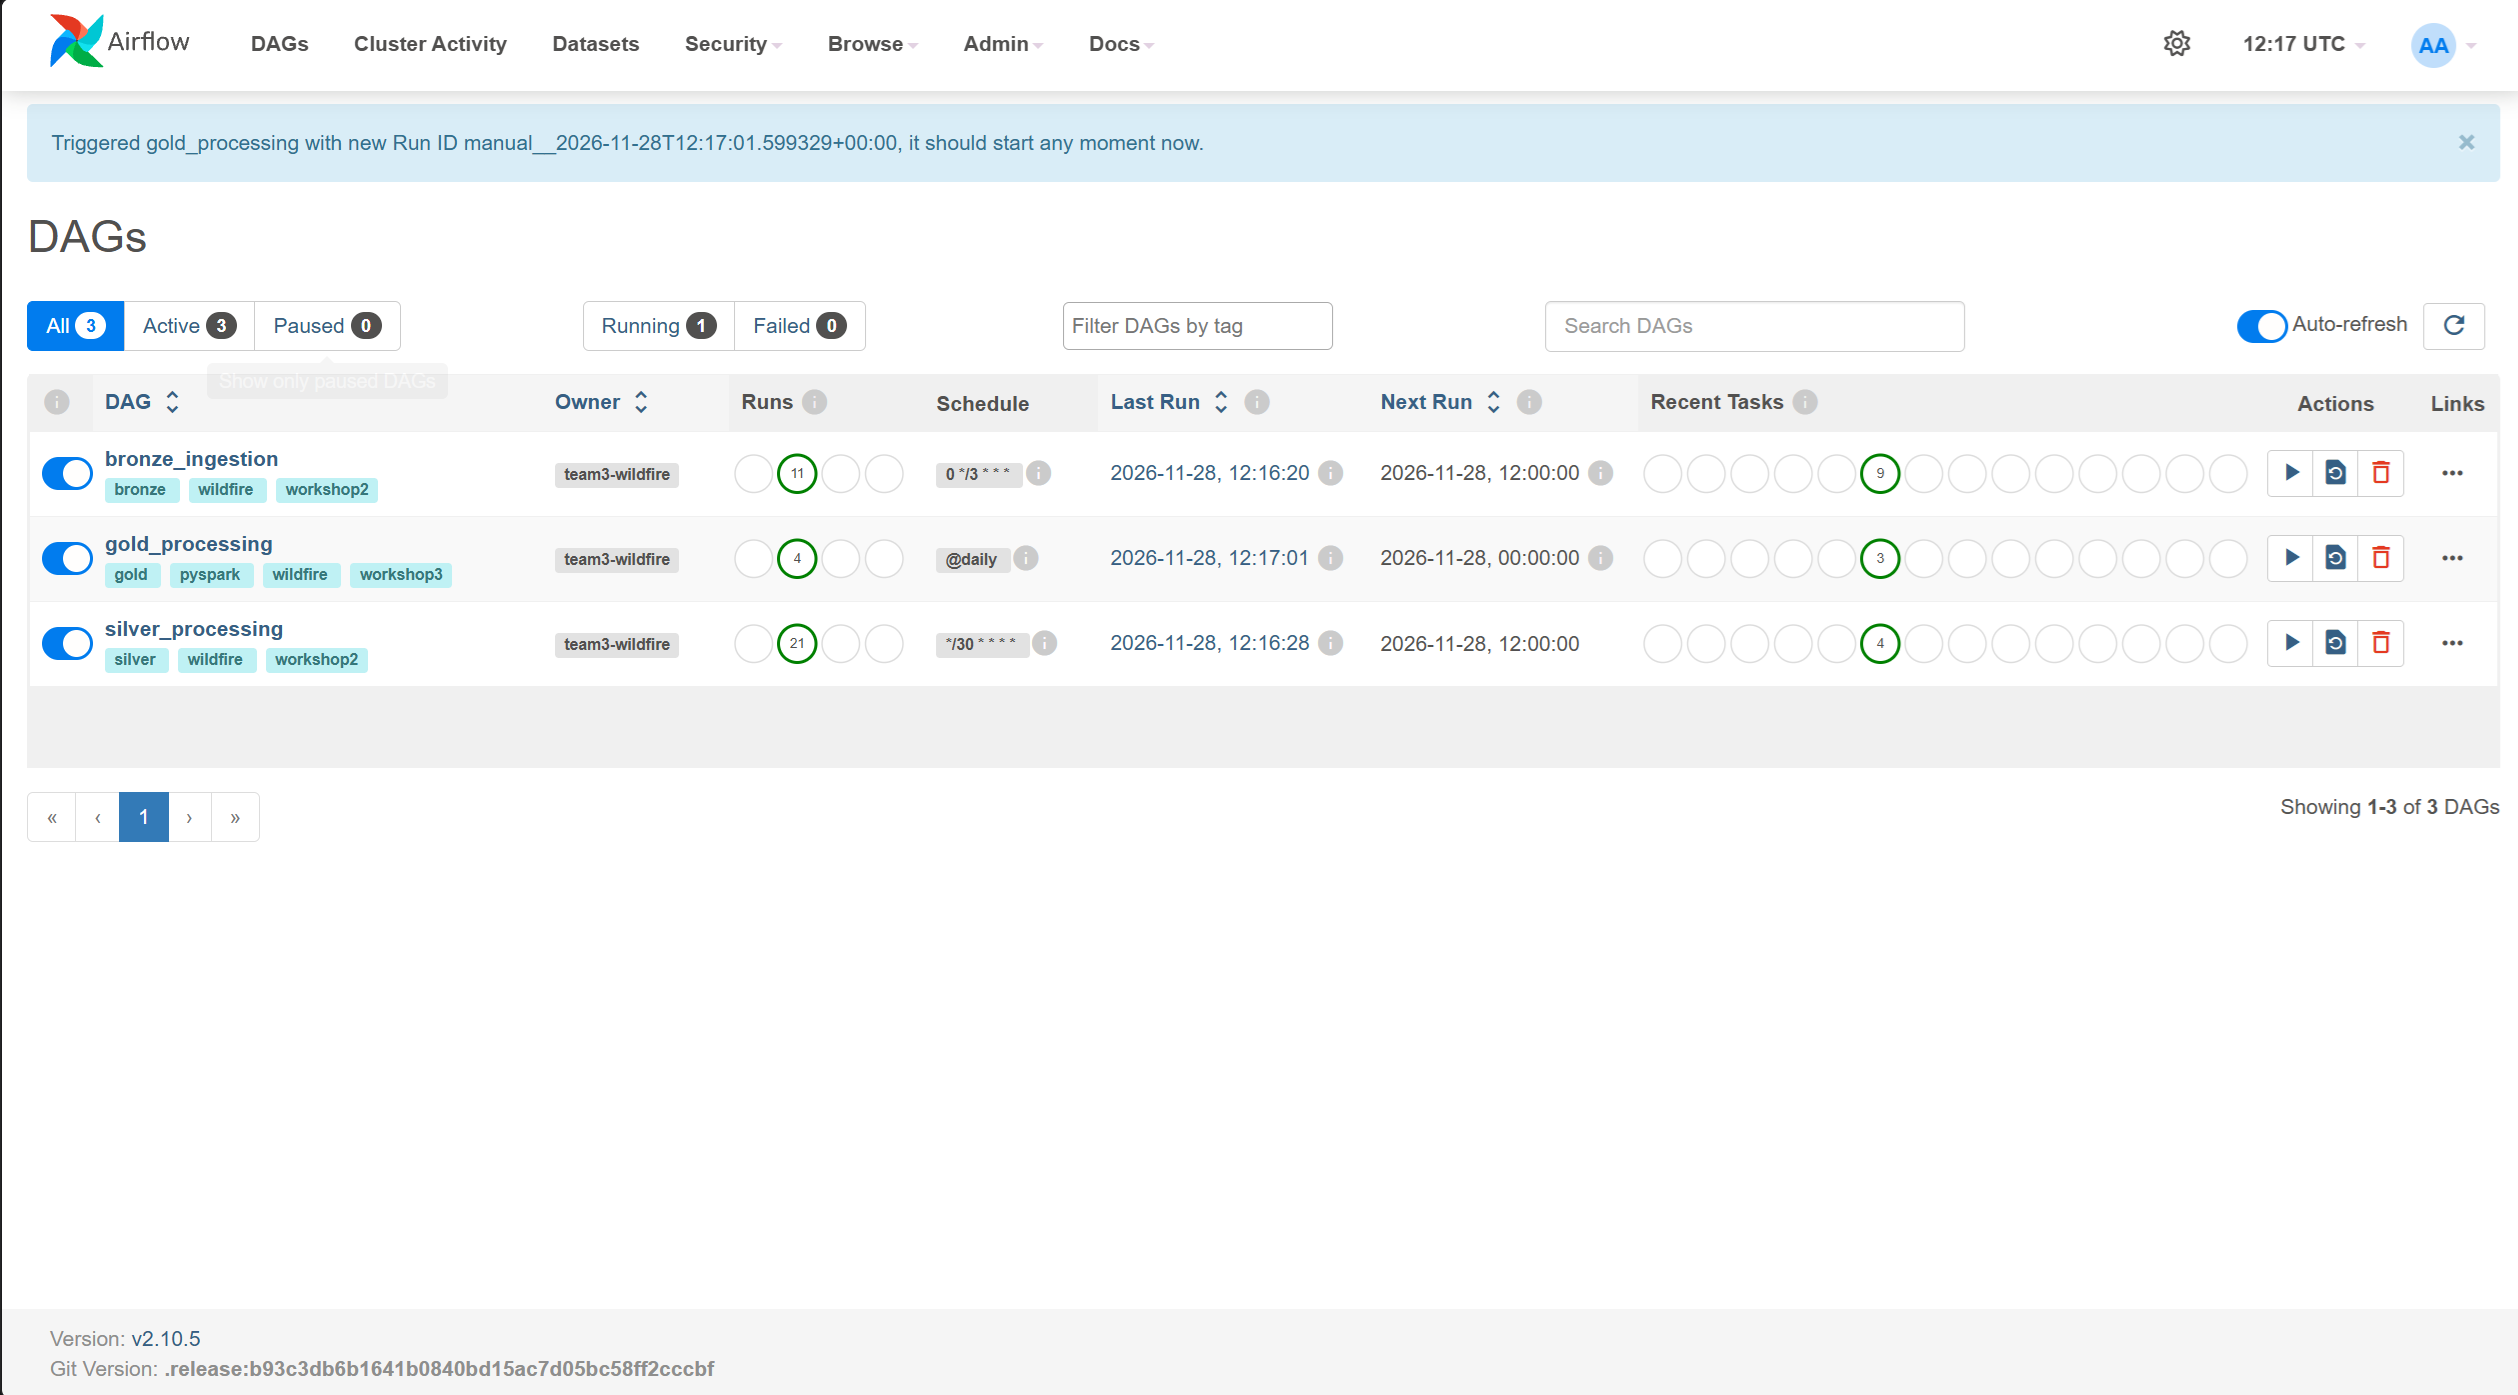
\includegraphics[width=0.95\textwidth, height=0.38\textheight, keepaspectratio]{screenshots/airflow_all_dags_success.png}
    \caption{Apache Airflow UI (\texttt{localhost:8080}) showing the three active Medallion DAGs (\texttt{bronze\_ingestion}, \texttt{silver\_processing}, and \texttt{gold\_processing}).}
    \label{fig:airflow}
\end{figure}

\subsection{Live Dashboards Populated with Gold Parquet Outputs}
Figures~\ref{fig:gov_dash} and~\ref{fig:story_dash} present full-page captures of both independent Plotly Dash web applications running locally on ports \texttt{8050} and \texttt{8051} directly over the Gold Parquet layer.

\begin{figure}[htbp]
    \centering
    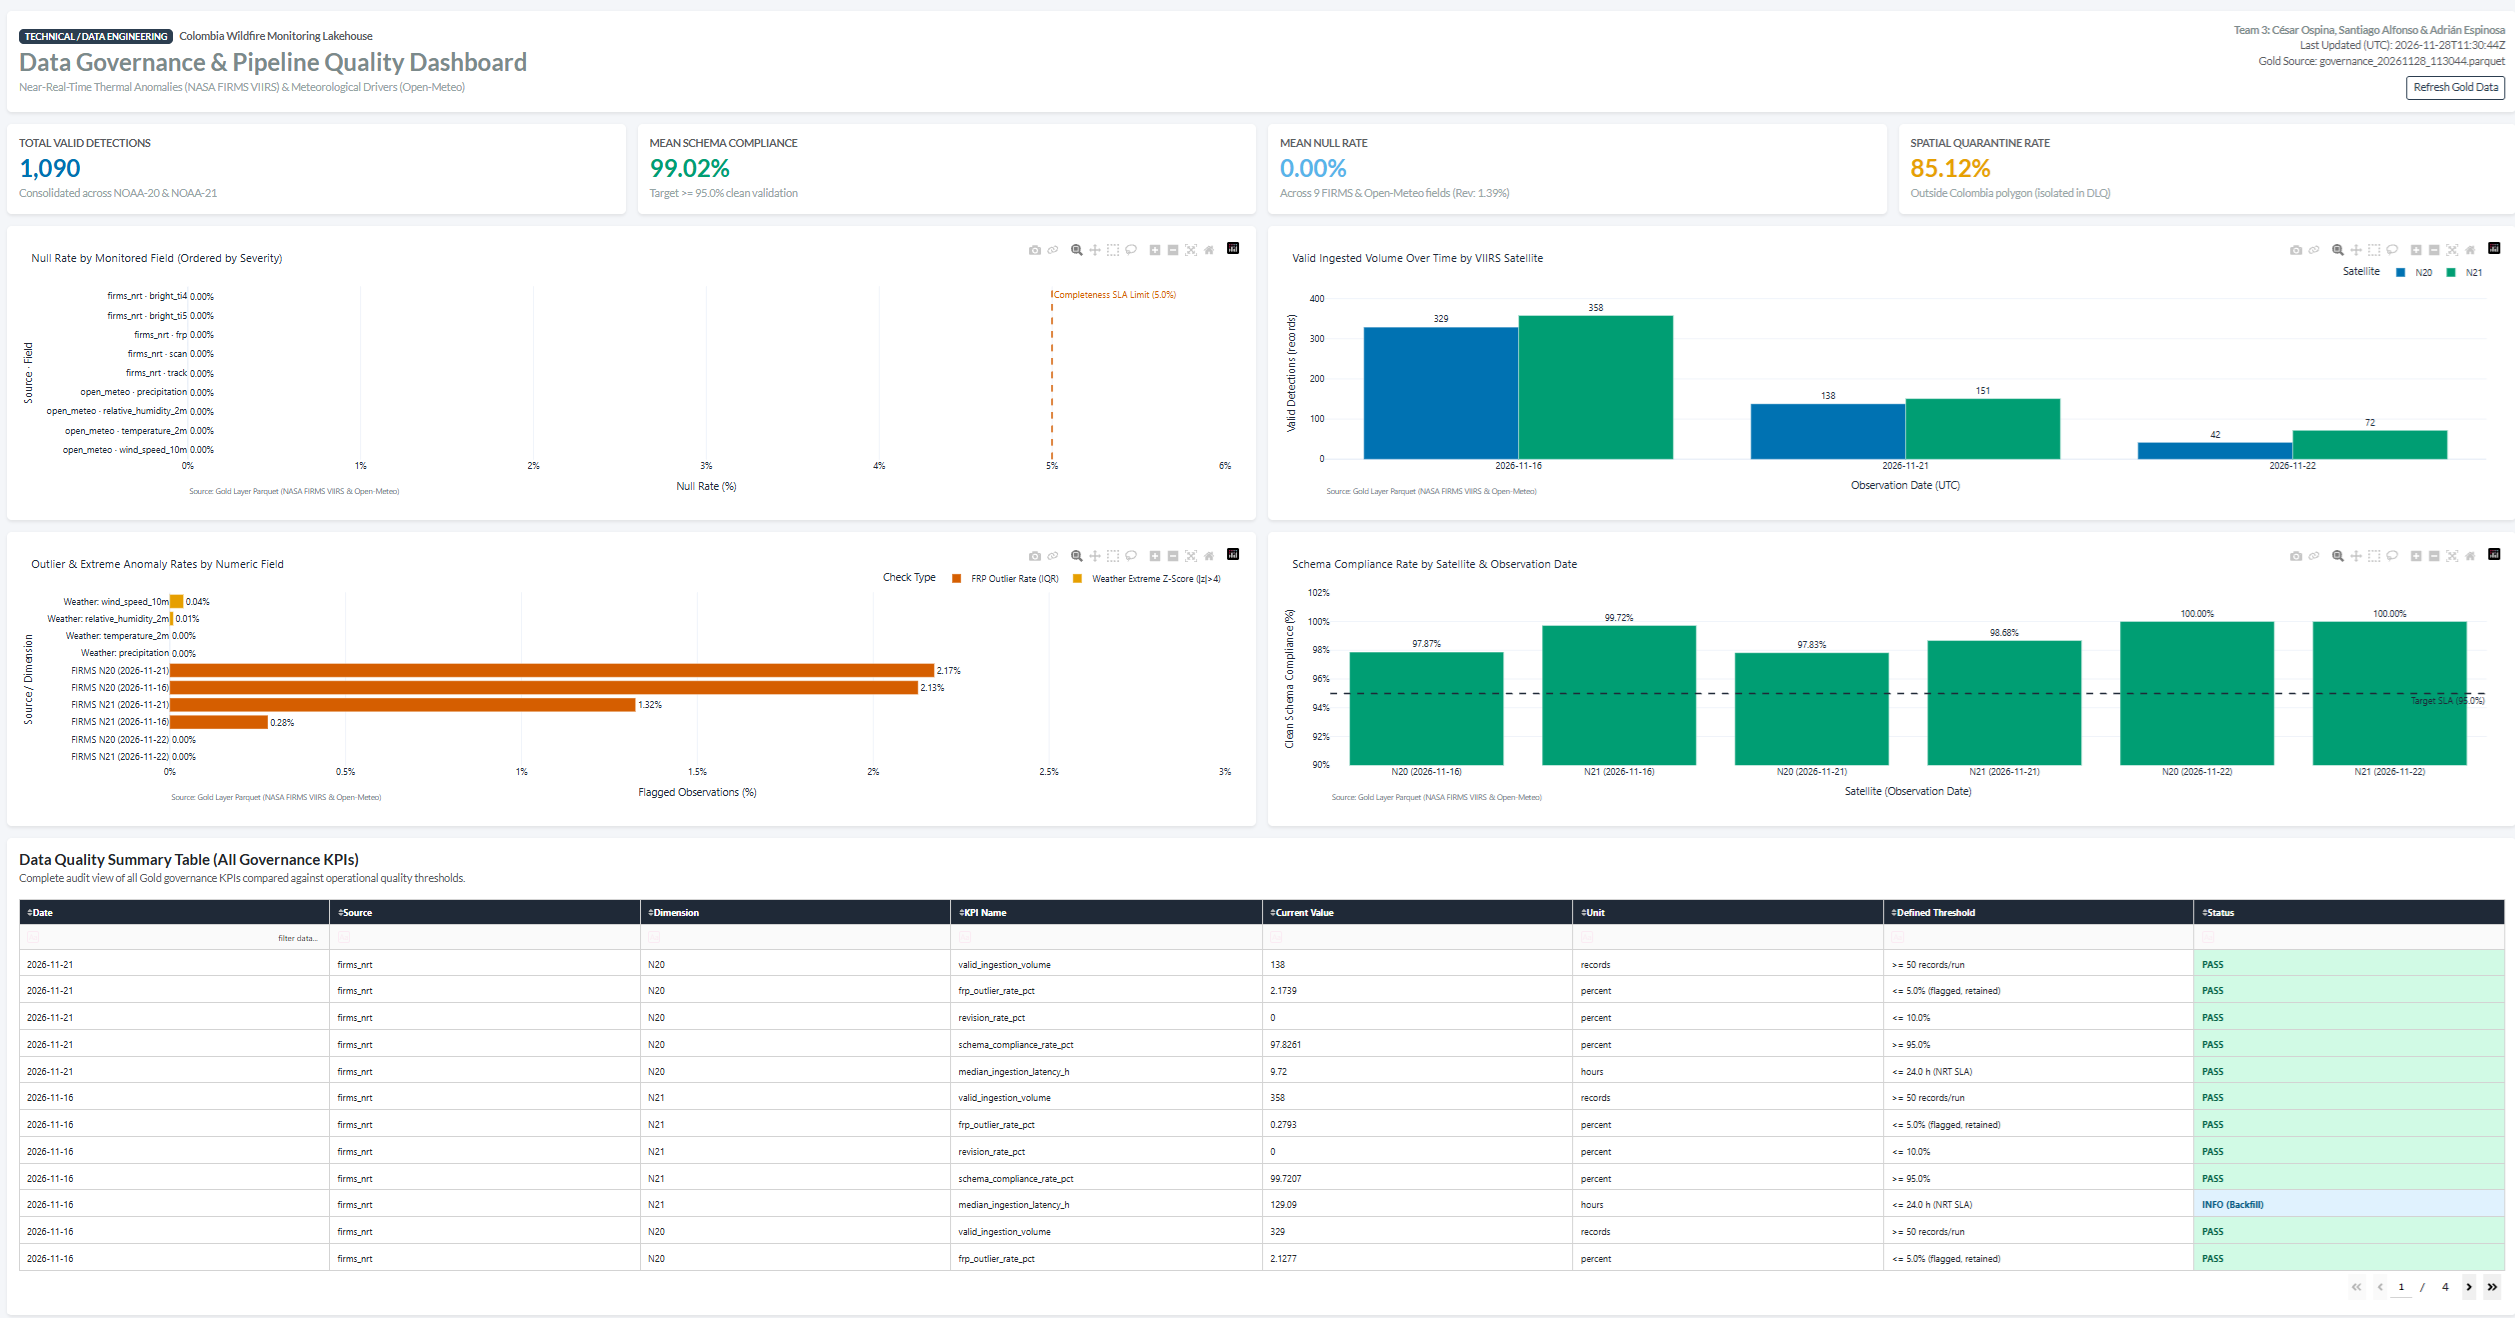
\includegraphics[width=0.95\textwidth, height=0.42\textheight, keepaspectratio]{screenshots/governance_dashboard_full.png}
    \caption{Full-page capture of the Data Governance \& Pipeline Quality Dashboard at \texttt{http://localhost:8050}.}
    \label{fig:gov_dash}
\end{figure}

\begin{figure}[htbp]
    \centering
    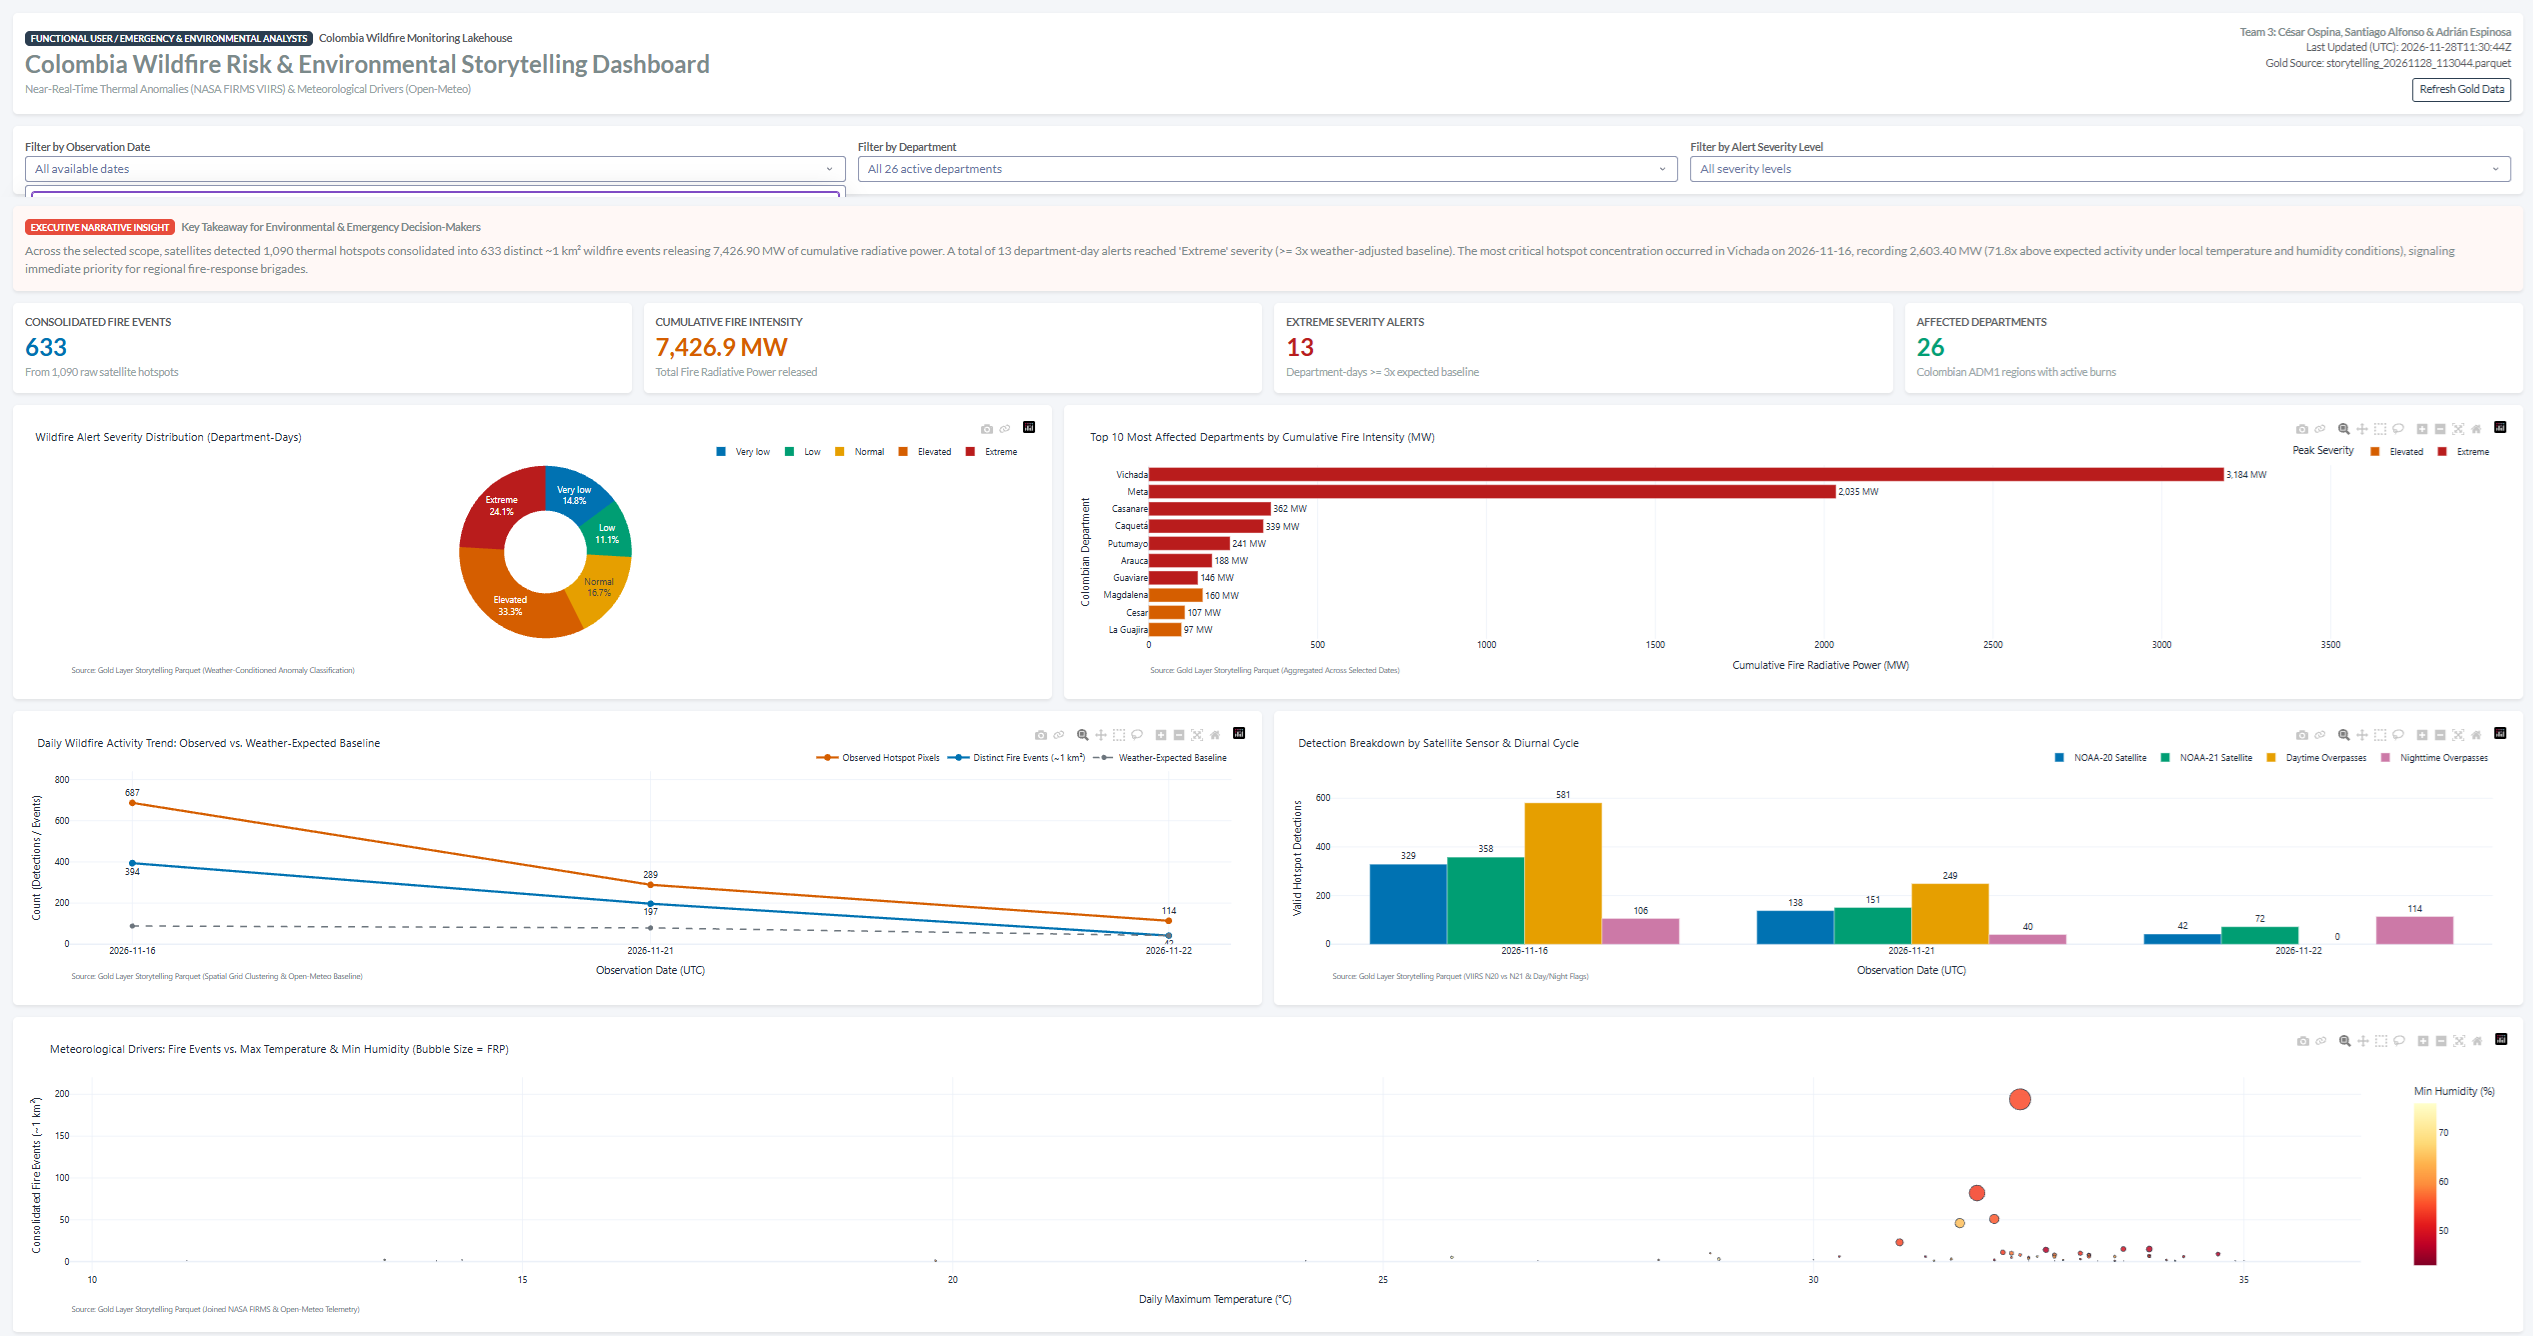
\includegraphics[width=0.95\textwidth, height=0.42\textheight, keepaspectratio]{screenshots/storytelling_dashboard_full.png}
    \caption{Full-page capture of the Colombia Wildfire Risk \& Environmental Storytelling Dashboard at \texttt{http://localhost:8051}.}
    \label{fig:story_dash}
\end{figure}

\FloatBarrier

\subsection{Repository Structure and Clean Reproduction}
Any external reviewer can clone the repository and reproduce the entire pipeline and both dashboards following \texttt{README.md}:

\begin{lstlisting}
wildfire-monitoring/
|-- airflow/dags/        # bronze_ingestion_dag.py, silver_processing_dag.py, gold_processing_dag.py
|-- dashboard/           # utils.py, governance_app.py (port 8050), storytelling_app.py (port 8051)
|-- datalake_bronze/     # Raw JSON envelopes with SHA-256 checksums
|-- datalake_silver/     # Validated Parquet partitions + _quarantine/ DLQ
|-- datalake_gold/       # PySpark Gold Parquet outputs (single source for Dash)
|-- src/pipeline/        # Ingestion, validation, spatial join & Gold PySpark modules
|-- workshop_4/          # Report LaTeX source, PDF & screenshots/ visual documentation
|-- docker-compose.yml   # Airflow 2.10.5 + Java 17/PySpark + PostGIS warehouse
|-- requirements.txt     # Pinned Dash, Plotly, Pandas, PyArrow & pipeline dependencies
`-- README.md            # Complete Docker, DAG execution & dashboard launch guide
\end{lstlisting}

\section{Challenges and Resolutions}

\begin{itemize}[leftmargin=1.4em, itemsep=3pt]
    \item \textbf{Pixel Over-Counting vs. Physical Fire Events:} Raw VIIRS satellite overpasses frequently flag multiple adjacent pixels over a single fire front. Consuming the Gold layer's $\sim 1\text{ km}^2$ spatial grid clustering (\texttt{fire\_event\_count}) distinguishes 633 physical fire events from 1,090 raw hotspot detections, preventing alarm inflation for decision-makers.
    \item \textbf{Historical Backfill Latency Classification:} Backfilled partitions (such as 2026-11-16 observations processed during end-to-end validation) naturally show ingestion latencies above the 24-hour near-real-time SLA (129.09 h). Rather than triggering false failure alerts, \texttt{governance\_app.py} labels latencies $> 24\text{ h}$ as \texttt{INFO (Backfill)} so genuine schema or completeness failures remain clearly visible.
    \item \textbf{Decoupled Multi-Port Execution:} Separating governance (\texttt{localhost:8050}) and storytelling (\texttt{localhost:8051}) into standalone Python modules sharing \texttt{dashboard/utils.py} keeps technical audits isolated from functional storytelling while maintaining strict single-source consumption of Gold Parquet files.
\end{itemize}

\begin{thebibliography}{9}
\bibitem{plotlydash}
Plotly Technologies Inc., \textit{Dash Python User Guide: Interactive Web Applications in Python}, 2026. Available: \url{https://dash.plotly.com/}

\bibitem{dbc}
Faculty.ai, \textit{Dash Bootstrap Components Documentation (v2.0)}, 2026. Available: \url{https://dash-bootstrap-components.opensource.faculty.ai/}

\bibitem{okabeito}
M. Okabe and K. Ito, ``Color Universal Design (CUD): How to make figures and presentations that are friendly to Colorblind people,'' J*FLY Data Depository for Drosophila Researchers, 2008.

\bibitem{few}
S. Few, \textit{Information Dashboard Design: Displaying Data for At-a-Glance Monitoring}, 2nd ed. Burlingame, CA, USA: Analytics Press, 2013.

\bibitem{firms}
NASA EOSDIS Land, Atmosphere Near real-time Capability for EOS (LANCE), \textit{Fire Information for Resource Management System (FIRMS) VIIRS Active Fire Data}, 2026. Available: \url{https://firms.modaps.eosdis.nasa.gov/}

\bibitem{openmeteo}
Open-Meteo, \textit{Open-Meteo Weather \& ERA5 Historical Telemetry API (CC-BY 4.0)}, 2026. Available: \url{https://open-meteo.com/}
\end{thebibliography}

\end{document}